\documentclass[twocolumn]{article}
\usepackage{graphicx}
\usepackage{amsmath}

\begin{document}
\title{Exercise 21 - Arctangen and Arccotangent}
\author{Simon Vendelbo Bylling Jensen}
\date{\today}
\maketitle

\begin{abstract}
The "Big programming exercise" solution of exercise 21. An implementation of Arctangent and Arccotangent using complementary and mutual recursion methods for a more efficient algoritm by solving their generating differential equation. 
\end{abstract}

\section{Problem description}
I have the student number 201507956, where 56 with modulus 35 (including the 0`th exercise) will give me exercise 21. This problem is regarding solving the generating differential equations for Arctangent and Arccotangent. The two differential equations to implement, i
\begin{align}
\arctan(x) &= \int_0^x \frac{1}{z^2 + 1} dz, \label{eq:arctan}\\
\mathrm{arccot}(x) &= \int_x^\infty \frac{1}{z^2 + 1} dz. \label{eq:arccot} 
\end{align}
This should at first be introduced, and reduced to numerical solution for $x > 0$. Afterwards by complimentary relation:
\begin{equation}
\arctan(x) + \mathrm{arccot}(x) = \frac{\pi}{2}.\label{eq:sumrelation}
\end{equation}
This should be implimented for most efficient calculation, by solving $\arctan(x)$, if $x \leq 1$, and $\mathrm{arccot}(x)$ for $x>1$. The algoritm should be done similarly to the error-function exercise by solution of the differnetial equation, which the integral equation represents. As an optional exercise, one can examine whether $x=1$ is the opmimal point to swich the integration routine.


\begin{figure}
% GNUPLOT: LaTeX picture with Postscript
\begingroup
  \makeatletter
  \providecommand\color[2][]{%
    \GenericError{(gnuplot) \space\space\space\@spaces}{%
      Package color not loaded in conjunction with
      terminal option `colourtext'%
    }{See the gnuplot documentation for explanation.%
    }{Either use 'blacktext' in gnuplot or load the package
      color.sty in LaTeX.}%
    \renewcommand\color[2][]{}%
  }%
  \providecommand\includegraphics[2][]{%
    \GenericError{(gnuplot) \space\space\space\@spaces}{%
      Package graphicx or graphics not loaded%
    }{See the gnuplot documentation for explanation.%
    }{The gnuplot epslatex terminal needs graphicx.sty or graphics.sty.}%
    \renewcommand\includegraphics[2][]{}%
  }%
  \providecommand\rotatebox[2]{#2}%
  \@ifundefined{ifGPcolor}{%
    \newif\ifGPcolor
    \GPcolortrue
  }{}%
  \@ifundefined{ifGPblacktext}{%
    \newif\ifGPblacktext
    \GPblacktexttrue
  }{}%
  % define a \g@addto@macro without @ in the name:
  \let\gplgaddtomacro\g@addto@macro
  % define empty templates for all commands taking text:
  \gdef\gplbacktext{}%
  \gdef\gplfronttext{}%
  \makeatother
  \ifGPblacktext
    % no textcolor at all
    \def\colorrgb#1{}%
    \def\colorgray#1{}%
  \else
    % gray or color?
    \ifGPcolor
      \def\colorrgb#1{\color[rgb]{#1}}%
      \def\colorgray#1{\color[gray]{#1}}%
      \expandafter\def\csname LTw\endcsname{\color{white}}%
      \expandafter\def\csname LTb\endcsname{\color{black}}%
      \expandafter\def\csname LTa\endcsname{\color{black}}%
      \expandafter\def\csname LT0\endcsname{\color[rgb]{1,0,0}}%
      \expandafter\def\csname LT1\endcsname{\color[rgb]{0,1,0}}%
      \expandafter\def\csname LT2\endcsname{\color[rgb]{0,0,1}}%
      \expandafter\def\csname LT3\endcsname{\color[rgb]{1,0,1}}%
      \expandafter\def\csname LT4\endcsname{\color[rgb]{0,1,1}}%
      \expandafter\def\csname LT5\endcsname{\color[rgb]{1,1,0}}%
      \expandafter\def\csname LT6\endcsname{\color[rgb]{0,0,0}}%
      \expandafter\def\csname LT7\endcsname{\color[rgb]{1,0.3,0}}%
      \expandafter\def\csname LT8\endcsname{\color[rgb]{0.5,0.5,0.5}}%
    \else
      % gray
      \def\colorrgb#1{\color{black}}%
      \def\colorgray#1{\color[gray]{#1}}%
      \expandafter\def\csname LTw\endcsname{\color{white}}%
      \expandafter\def\csname LTb\endcsname{\color{black}}%
      \expandafter\def\csname LTa\endcsname{\color{black}}%
      \expandafter\def\csname LT0\endcsname{\color{black}}%
      \expandafter\def\csname LT1\endcsname{\color{black}}%
      \expandafter\def\csname LT2\endcsname{\color{black}}%
      \expandafter\def\csname LT3\endcsname{\color{black}}%
      \expandafter\def\csname LT4\endcsname{\color{black}}%
      \expandafter\def\csname LT5\endcsname{\color{black}}%
      \expandafter\def\csname LT6\endcsname{\color{black}}%
      \expandafter\def\csname LT7\endcsname{\color{black}}%
      \expandafter\def\csname LT8\endcsname{\color{black}}%
    \fi
  \fi
    \setlength{\unitlength}{0.0500bp}%
    \ifx\gptboxheight\undefined%
      \newlength{\gptboxheight}%
      \newlength{\gptboxwidth}%
      \newsavebox{\gptboxtext}%
    \fi%
    \setlength{\fboxrule}{0.5pt}%
    \setlength{\fboxsep}{1pt}%
\begin{picture}(4320.00,3456.00)%
    \gplgaddtomacro\gplbacktext{%
      \csname LTb\endcsname%%
      \put(645,669){\makebox(0,0)[r]{\strut{}$0$}}%
      \csname LTb\endcsname%%
      \put(645,994){\makebox(0,0)[r]{\strut{}$100$}}%
      \csname LTb\endcsname%%
      \put(645,1319){\makebox(0,0)[r]{\strut{}$200$}}%
      \csname LTb\endcsname%%
      \put(645,1644){\makebox(0,0)[r]{\strut{}$300$}}%
      \csname LTb\endcsname%%
      \put(645,1969){\makebox(0,0)[r]{\strut{}$400$}}%
      \csname LTb\endcsname%%
      \put(645,2294){\makebox(0,0)[r]{\strut{}$500$}}%
      \csname LTb\endcsname%%
      \put(645,2619){\makebox(0,0)[r]{\strut{}$600$}}%
      \csname LTb\endcsname%%
      \put(645,2944){\makebox(0,0)[r]{\strut{}$700$}}%
      \csname LTb\endcsname%%
      \put(645,3269){\makebox(0,0)[r]{\strut{}$800$}}%
      \csname LTb\endcsname%%
      \put(821,409){\makebox(0,0){\strut{}$0$}}%
      \csname LTb\endcsname%%
      \put(1341,409){\makebox(0,0){\strut{}$5$}}%
      \csname LTb\endcsname%%
      \put(1860,409){\makebox(0,0){\strut{}$10$}}%
      \csname LTb\endcsname%%
      \put(2380,409){\makebox(0,0){\strut{}$15$}}%
      \csname LTb\endcsname%%
      \put(2900,409){\makebox(0,0){\strut{}$20$}}%
      \csname LTb\endcsname%%
      \put(3419,409){\makebox(0,0){\strut{}$25$}}%
      \csname LTb\endcsname%%
      \put(3939,409){\makebox(0,0){\strut{}$30$}}%
    }%
    \gplgaddtomacro\gplfronttext{%
      \csname LTb\endcsname%%
      \put(153,1969){\rotatebox{-270}{\makebox(0,0){\strut{}Number of Iterations}}}%
      \csname LTb\endcsname%%
      \put(2380,130){\makebox(0,0){\strut{}Matrix Dimension "n"}}%
      \csname LTb\endcsname%%
      \put(3065,3102){\makebox(0,0)[r]{\strut{}Power Iter.}}%
      \csname LTb\endcsname%%
      \put(3065,2916){\makebox(0,0)[r]{\strut{}Inverse Power Iter.}}%
      \csname LTb\endcsname%%
      \put(3065,2730){\makebox(0,0)[r]{\strut{}Shifted Inverse Iter.}}%
      \csname LTb\endcsname%%
      \put(3065,2544){\makebox(0,0)[r]{\strut{}Inverse Iter.}}%
    }%
    \gplbacktext
    \put(0,0){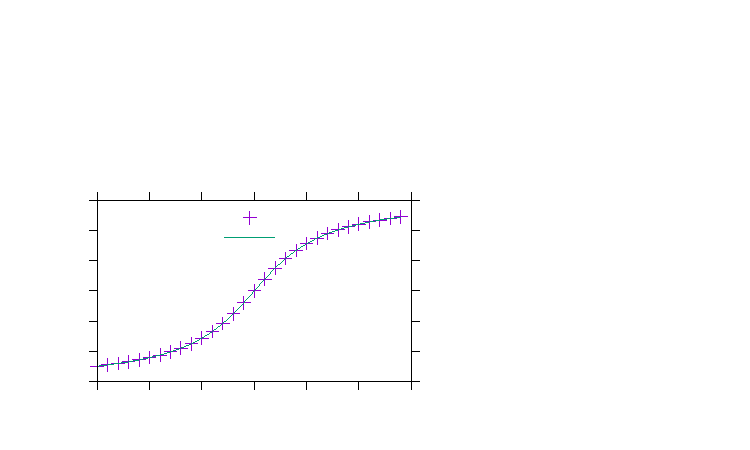
\includegraphics{plot-cairo}}%
    \gplfronttext
  \end{picture}%
\endgroup

\caption{Comparison between the calculated arctangent function using the differential equation found in "myarctan.c" and the arctangent function from the math.h library.}
\label{fig-atan}
\end{figure}

\begin{figure}
% GNUPLOT: LaTeX picture with Postscript
\begingroup
  \makeatletter
  \providecommand\color[2][]{%
    \GenericError{(gnuplot) \space\space\space\@spaces}{%
      Package color not loaded in conjunction with
      terminal option `colourtext'%
    }{See the gnuplot documentation for explanation.%
    }{Either use 'blacktext' in gnuplot or load the package
      color.sty in LaTeX.}%
    \renewcommand\color[2][]{}%
  }%
  \providecommand\includegraphics[2][]{%
    \GenericError{(gnuplot) \space\space\space\@spaces}{%
      Package graphicx or graphics not loaded%
    }{See the gnuplot documentation for explanation.%
    }{The gnuplot epslatex terminal needs graphicx.sty or graphics.sty.}%
    \renewcommand\includegraphics[2][]{}%
  }%
  \providecommand\rotatebox[2]{#2}%
  \@ifundefined{ifGPcolor}{%
    \newif\ifGPcolor
    \GPcolortrue
  }{}%
  \@ifundefined{ifGPblacktext}{%
    \newif\ifGPblacktext
    \GPblacktexttrue
  }{}%
  % define a \g@addto@macro without @ in the name:
  \let\gplgaddtomacro\g@addto@macro
  % define empty templates for all commands taking text:
  \gdef\gplbacktext{}%
  \gdef\gplfronttext{}%
  \makeatother
  \ifGPblacktext
    % no textcolor at all
    \def\colorrgb#1{}%
    \def\colorgray#1{}%
  \else
    % gray or color?
    \ifGPcolor
      \def\colorrgb#1{\color[rgb]{#1}}%
      \def\colorgray#1{\color[gray]{#1}}%
      \expandafter\def\csname LTw\endcsname{\color{white}}%
      \expandafter\def\csname LTb\endcsname{\color{black}}%
      \expandafter\def\csname LTa\endcsname{\color{black}}%
      \expandafter\def\csname LT0\endcsname{\color[rgb]{1,0,0}}%
      \expandafter\def\csname LT1\endcsname{\color[rgb]{0,1,0}}%
      \expandafter\def\csname LT2\endcsname{\color[rgb]{0,0,1}}%
      \expandafter\def\csname LT3\endcsname{\color[rgb]{1,0,1}}%
      \expandafter\def\csname LT4\endcsname{\color[rgb]{0,1,1}}%
      \expandafter\def\csname LT5\endcsname{\color[rgb]{1,1,0}}%
      \expandafter\def\csname LT6\endcsname{\color[rgb]{0,0,0}}%
      \expandafter\def\csname LT7\endcsname{\color[rgb]{1,0.3,0}}%
      \expandafter\def\csname LT8\endcsname{\color[rgb]{0.5,0.5,0.5}}%
    \else
      % gray
      \def\colorrgb#1{\color{black}}%
      \def\colorgray#1{\color[gray]{#1}}%
      \expandafter\def\csname LTw\endcsname{\color{white}}%
      \expandafter\def\csname LTb\endcsname{\color{black}}%
      \expandafter\def\csname LTa\endcsname{\color{black}}%
      \expandafter\def\csname LT0\endcsname{\color{black}}%
      \expandafter\def\csname LT1\endcsname{\color{black}}%
      \expandafter\def\csname LT2\endcsname{\color{black}}%
      \expandafter\def\csname LT3\endcsname{\color{black}}%
      \expandafter\def\csname LT4\endcsname{\color{black}}%
      \expandafter\def\csname LT5\endcsname{\color{black}}%
      \expandafter\def\csname LT6\endcsname{\color{black}}%
      \expandafter\def\csname LT7\endcsname{\color{black}}%
      \expandafter\def\csname LT8\endcsname{\color{black}}%
    \fi
  \fi
    \setlength{\unitlength}{0.0500bp}%
    \ifx\gptboxheight\undefined%
      \newlength{\gptboxheight}%
      \newlength{\gptboxwidth}%
      \newsavebox{\gptboxtext}%
    \fi%
    \setlength{\fboxrule}{0.5pt}%
    \setlength{\fboxsep}{1pt}%
\begin{picture}(4320.00,2592.00)%
    \gplgaddtomacro\gplbacktext{%
      \csname LTb\endcsname%%
      \put(747,669){\makebox(0,0)[r]{\strut{}$-1.5$}}%
      \csname LTb\endcsname%%
      \put(747,917){\makebox(0,0)[r]{\strut{}$-1$}}%
      \csname LTb\endcsname%%
      \put(747,1165){\makebox(0,0)[r]{\strut{}$-0.5$}}%
      \csname LTb\endcsname%%
      \put(747,1413){\makebox(0,0)[r]{\strut{}$0$}}%
      \csname LTb\endcsname%%
      \put(747,1661){\makebox(0,0)[r]{\strut{}$0.5$}}%
      \csname LTb\endcsname%%
      \put(747,1909){\makebox(0,0)[r]{\strut{}$1$}}%
      \csname LTb\endcsname%%
      \put(747,2157){\makebox(0,0)[r]{\strut{}$1.5$}}%
      \csname LTb\endcsname%%
      \put(747,2405){\makebox(0,0)[r]{\strut{}$2$}}%
      \csname LTb\endcsname%%
      \put(923,409){\makebox(0,0){\strut{}$-3$}}%
      \csname LTb\endcsname%%
      \put(1426,409){\makebox(0,0){\strut{}$-2$}}%
      \csname LTb\endcsname%%
      \put(1928,409){\makebox(0,0){\strut{}$-1$}}%
      \csname LTb\endcsname%%
      \put(2431,409){\makebox(0,0){\strut{}$0$}}%
      \csname LTb\endcsname%%
      \put(2934,409){\makebox(0,0){\strut{}$1$}}%
      \csname LTb\endcsname%%
      \put(3436,409){\makebox(0,0){\strut{}$2$}}%
      \csname LTb\endcsname%%
      \put(3939,409){\makebox(0,0){\strut{}$3$}}%
    }%
    \gplgaddtomacro\gplfronttext{%
      \csname LTb\endcsname%%
      \put(153,1537){\rotatebox{-270}{\makebox(0,0){\strut{}y}}}%
      \csname LTb\endcsname%%
      \put(2431,130){\makebox(0,0){\strut{}x}}%
      \csname LTb\endcsname%%
      \put(3151,2238){\makebox(0,0)[r]{\strut{}calculated}}%
      \csname LTb\endcsname%%
      \put(3151,2052){\makebox(0,0)[r]{\strut{}exact}}%
    }%
    \gplbacktext
    \put(0,0){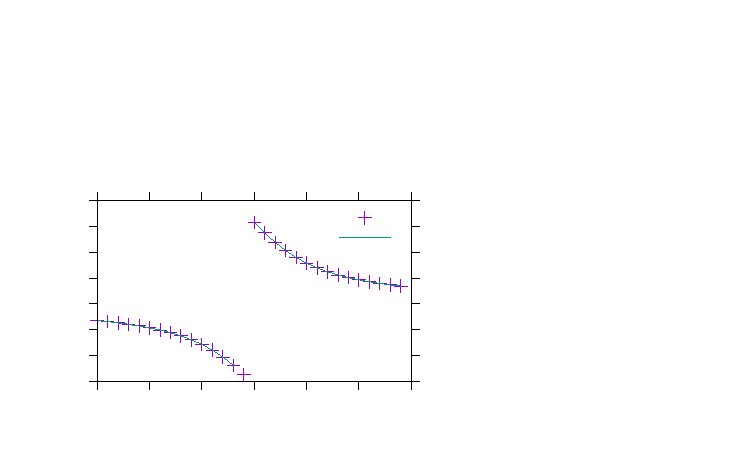
\includegraphics{plot-cairo2}}%
    \gplfronttext
  \end{picture}%
\endgroup

\caption{Comparison between the calculated arccotangent function using the differential equation found in "myarccot.c" and the arccot function from the math.h library, by calculation of arctan of the inverse value.}
\label{fig-acot}
\end{figure}

\begin{figure}
% GNUPLOT: LaTeX picture with Postscript
\begingroup
  \makeatletter
  \providecommand\color[2][]{%
    \GenericError{(gnuplot) \space\space\space\@spaces}{%
      Package color not loaded in conjunction with
      terminal option `colourtext'%
    }{See the gnuplot documentation for explanation.%
    }{Either use 'blacktext' in gnuplot or load the package
      color.sty in LaTeX.}%
    \renewcommand\color[2][]{}%
  }%
  \providecommand\includegraphics[2][]{%
    \GenericError{(gnuplot) \space\space\space\@spaces}{%
      Package graphicx or graphics not loaded%
    }{See the gnuplot documentation for explanation.%
    }{The gnuplot epslatex terminal needs graphicx.sty or graphics.sty.}%
    \renewcommand\includegraphics[2][]{}%
  }%
  \providecommand\rotatebox[2]{#2}%
  \@ifundefined{ifGPcolor}{%
    \newif\ifGPcolor
    \GPcolortrue
  }{}%
  \@ifundefined{ifGPblacktext}{%
    \newif\ifGPblacktext
    \GPblacktexttrue
  }{}%
  % define a \g@addto@macro without @ in the name:
  \let\gplgaddtomacro\g@addto@macro
  % define empty templates for all commands taking text:
  \gdef\gplbacktext{}%
  \gdef\gplfronttext{}%
  \makeatother
  \ifGPblacktext
    % no textcolor at all
    \def\colorrgb#1{}%
    \def\colorgray#1{}%
  \else
    % gray or color?
    \ifGPcolor
      \def\colorrgb#1{\color[rgb]{#1}}%
      \def\colorgray#1{\color[gray]{#1}}%
      \expandafter\def\csname LTw\endcsname{\color{white}}%
      \expandafter\def\csname LTb\endcsname{\color{black}}%
      \expandafter\def\csname LTa\endcsname{\color{black}}%
      \expandafter\def\csname LT0\endcsname{\color[rgb]{1,0,0}}%
      \expandafter\def\csname LT1\endcsname{\color[rgb]{0,1,0}}%
      \expandafter\def\csname LT2\endcsname{\color[rgb]{0,0,1}}%
      \expandafter\def\csname LT3\endcsname{\color[rgb]{1,0,1}}%
      \expandafter\def\csname LT4\endcsname{\color[rgb]{0,1,1}}%
      \expandafter\def\csname LT5\endcsname{\color[rgb]{1,1,0}}%
      \expandafter\def\csname LT6\endcsname{\color[rgb]{0,0,0}}%
      \expandafter\def\csname LT7\endcsname{\color[rgb]{1,0.3,0}}%
      \expandafter\def\csname LT8\endcsname{\color[rgb]{0.5,0.5,0.5}}%
    \else
      % gray
      \def\colorrgb#1{\color{black}}%
      \def\colorgray#1{\color[gray]{#1}}%
      \expandafter\def\csname LTw\endcsname{\color{white}}%
      \expandafter\def\csname LTb\endcsname{\color{black}}%
      \expandafter\def\csname LTa\endcsname{\color{black}}%
      \expandafter\def\csname LT0\endcsname{\color{black}}%
      \expandafter\def\csname LT1\endcsname{\color{black}}%
      \expandafter\def\csname LT2\endcsname{\color{black}}%
      \expandafter\def\csname LT3\endcsname{\color{black}}%
      \expandafter\def\csname LT4\endcsname{\color{black}}%
      \expandafter\def\csname LT5\endcsname{\color{black}}%
      \expandafter\def\csname LT6\endcsname{\color{black}}%
      \expandafter\def\csname LT7\endcsname{\color{black}}%
      \expandafter\def\csname LT8\endcsname{\color{black}}%
    \fi
  \fi
    \setlength{\unitlength}{0.0500bp}%
    \ifx\gptboxheight\undefined%
      \newlength{\gptboxheight}%
      \newlength{\gptboxwidth}%
      \newsavebox{\gptboxtext}%
    \fi%
    \setlength{\fboxrule}{0.5pt}%
    \setlength{\fboxsep}{1pt}%
\begin{picture}(4320.00,2592.00)%
    \gplgaddtomacro\gplbacktext{%
      \csname LTb\endcsname%%
      \put(747,669){\makebox(0,0)[r]{\strut{}$-1.5$}}%
      \csname LTb\endcsname%%
      \put(747,958){\makebox(0,0)[r]{\strut{}$-1$}}%
      \csname LTb\endcsname%%
      \put(747,1248){\makebox(0,0)[r]{\strut{}$-0.5$}}%
      \csname LTb\endcsname%%
      \put(747,1537){\makebox(0,0)[r]{\strut{}$0$}}%
      \csname LTb\endcsname%%
      \put(747,1826){\makebox(0,0)[r]{\strut{}$0.5$}}%
      \csname LTb\endcsname%%
      \put(747,2116){\makebox(0,0)[r]{\strut{}$1$}}%
      \csname LTb\endcsname%%
      \put(747,2405){\makebox(0,0)[r]{\strut{}$1.5$}}%
      \csname LTb\endcsname%%
      \put(923,409){\makebox(0,0){\strut{}$-3$}}%
      \csname LTb\endcsname%%
      \put(1426,409){\makebox(0,0){\strut{}$-2$}}%
      \csname LTb\endcsname%%
      \put(1928,409){\makebox(0,0){\strut{}$-1$}}%
      \csname LTb\endcsname%%
      \put(2431,409){\makebox(0,0){\strut{}$0$}}%
      \csname LTb\endcsname%%
      \put(2934,409){\makebox(0,0){\strut{}$1$}}%
      \csname LTb\endcsname%%
      \put(3436,409){\makebox(0,0){\strut{}$2$}}%
      \csname LTb\endcsname%%
      \put(3939,409){\makebox(0,0){\strut{}$3$}}%
    }%
    \gplgaddtomacro\gplfronttext{%
      \csname LTb\endcsname%%
      \put(153,1537){\rotatebox{-270}{\makebox(0,0){\strut{}y}}}%
      \csname LTb\endcsname%%
      \put(2431,130){\makebox(0,0){\strut{}x}}%
      \csname LTb\endcsname%%
      \put(3151,2238){\makebox(0,0)[r]{\strut{}calculated}}%
      \csname LTb\endcsname%%
      \put(3151,2052){\makebox(0,0)[r]{\strut{}exact}}%
    }%
    \gplbacktext
    \put(0,0){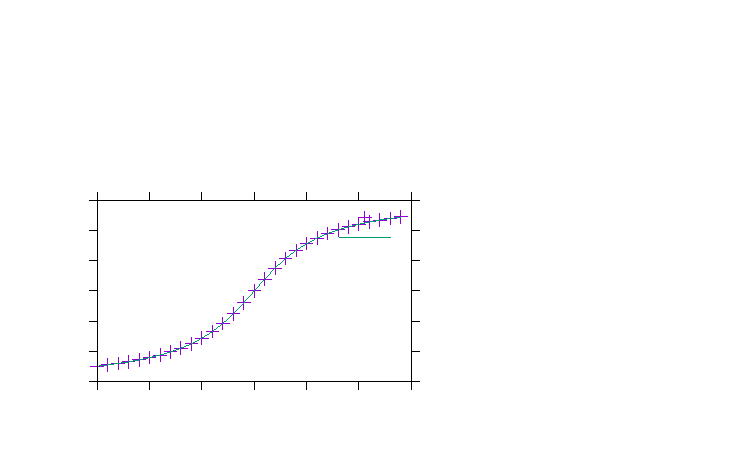
\includegraphics{plot-cairo3}}%
    \gplfronttext
  \end{picture}%
\endgroup

\caption{Comparison between the calculated modified arctangent function using differential equation found in "myarctan2.c" and the artangent function from the math.h library.}
\label{fig-atan2}
\end{figure}

\begin{figure}
% GNUPLOT: LaTeX picture with Postscript
\begingroup
  \makeatletter
  \providecommand\color[2][]{%
    \GenericError{(gnuplot) \space\space\space\@spaces}{%
      Package color not loaded in conjunction with
      terminal option `colourtext'%
    }{See the gnuplot documentation for explanation.%
    }{Either use 'blacktext' in gnuplot or load the package
      color.sty in LaTeX.}%
    \renewcommand\color[2][]{}%
  }%
  \providecommand\includegraphics[2][]{%
    \GenericError{(gnuplot) \space\space\space\@spaces}{%
      Package graphicx or graphics not loaded%
    }{See the gnuplot documentation for explanation.%
    }{The gnuplot epslatex terminal needs graphicx.sty or graphics.sty.}%
    \renewcommand\includegraphics[2][]{}%
  }%
  \providecommand\rotatebox[2]{#2}%
  \@ifundefined{ifGPcolor}{%
    \newif\ifGPcolor
    \GPcolortrue
  }{}%
  \@ifundefined{ifGPblacktext}{%
    \newif\ifGPblacktext
    \GPblacktexttrue
  }{}%
  % define a \g@addto@macro without @ in the name:
  \let\gplgaddtomacro\g@addto@macro
  % define empty templates for all commands taking text:
  \gdef\gplbacktext{}%
  \gdef\gplfronttext{}%
  \makeatother
  \ifGPblacktext
    % no textcolor at all
    \def\colorrgb#1{}%
    \def\colorgray#1{}%
  \else
    % gray or color?
    \ifGPcolor
      \def\colorrgb#1{\color[rgb]{#1}}%
      \def\colorgray#1{\color[gray]{#1}}%
      \expandafter\def\csname LTw\endcsname{\color{white}}%
      \expandafter\def\csname LTb\endcsname{\color{black}}%
      \expandafter\def\csname LTa\endcsname{\color{black}}%
      \expandafter\def\csname LT0\endcsname{\color[rgb]{1,0,0}}%
      \expandafter\def\csname LT1\endcsname{\color[rgb]{0,1,0}}%
      \expandafter\def\csname LT2\endcsname{\color[rgb]{0,0,1}}%
      \expandafter\def\csname LT3\endcsname{\color[rgb]{1,0,1}}%
      \expandafter\def\csname LT4\endcsname{\color[rgb]{0,1,1}}%
      \expandafter\def\csname LT5\endcsname{\color[rgb]{1,1,0}}%
      \expandafter\def\csname LT6\endcsname{\color[rgb]{0,0,0}}%
      \expandafter\def\csname LT7\endcsname{\color[rgb]{1,0.3,0}}%
      \expandafter\def\csname LT8\endcsname{\color[rgb]{0.5,0.5,0.5}}%
    \else
      % gray
      \def\colorrgb#1{\color{black}}%
      \def\colorgray#1{\color[gray]{#1}}%
      \expandafter\def\csname LTw\endcsname{\color{white}}%
      \expandafter\def\csname LTb\endcsname{\color{black}}%
      \expandafter\def\csname LTa\endcsname{\color{black}}%
      \expandafter\def\csname LT0\endcsname{\color{black}}%
      \expandafter\def\csname LT1\endcsname{\color{black}}%
      \expandafter\def\csname LT2\endcsname{\color{black}}%
      \expandafter\def\csname LT3\endcsname{\color{black}}%
      \expandafter\def\csname LT4\endcsname{\color{black}}%
      \expandafter\def\csname LT5\endcsname{\color{black}}%
      \expandafter\def\csname LT6\endcsname{\color{black}}%
      \expandafter\def\csname LT7\endcsname{\color{black}}%
      \expandafter\def\csname LT8\endcsname{\color{black}}%
    \fi
  \fi
    \setlength{\unitlength}{0.0500bp}%
    \ifx\gptboxheight\undefined%
      \newlength{\gptboxheight}%
      \newlength{\gptboxwidth}%
      \newsavebox{\gptboxtext}%
    \fi%
    \setlength{\fboxrule}{0.5pt}%
    \setlength{\fboxsep}{1pt}%
\begin{picture}(4320.00,2592.00)%
    \gplgaddtomacro\gplbacktext{%
      \csname LTb\endcsname%%
      \put(747,669){\makebox(0,0)[r]{\strut{}$-1.5$}}%
      \csname LTb\endcsname%%
      \put(747,917){\makebox(0,0)[r]{\strut{}$-1$}}%
      \csname LTb\endcsname%%
      \put(747,1165){\makebox(0,0)[r]{\strut{}$-0.5$}}%
      \csname LTb\endcsname%%
      \put(747,1413){\makebox(0,0)[r]{\strut{}$0$}}%
      \csname LTb\endcsname%%
      \put(747,1661){\makebox(0,0)[r]{\strut{}$0.5$}}%
      \csname LTb\endcsname%%
      \put(747,1909){\makebox(0,0)[r]{\strut{}$1$}}%
      \csname LTb\endcsname%%
      \put(747,2157){\makebox(0,0)[r]{\strut{}$1.5$}}%
      \csname LTb\endcsname%%
      \put(747,2405){\makebox(0,0)[r]{\strut{}$2$}}%
      \csname LTb\endcsname%%
      \put(923,409){\makebox(0,0){\strut{}$-3$}}%
      \csname LTb\endcsname%%
      \put(1426,409){\makebox(0,0){\strut{}$-2$}}%
      \csname LTb\endcsname%%
      \put(1928,409){\makebox(0,0){\strut{}$-1$}}%
      \csname LTb\endcsname%%
      \put(2431,409){\makebox(0,0){\strut{}$0$}}%
      \csname LTb\endcsname%%
      \put(2934,409){\makebox(0,0){\strut{}$1$}}%
      \csname LTb\endcsname%%
      \put(3436,409){\makebox(0,0){\strut{}$2$}}%
      \csname LTb\endcsname%%
      \put(3939,409){\makebox(0,0){\strut{}$3$}}%
    }%
    \gplgaddtomacro\gplfronttext{%
      \csname LTb\endcsname%%
      \put(153,1537){\rotatebox{-270}{\makebox(0,0){\strut{}y}}}%
      \csname LTb\endcsname%%
      \put(2431,130){\makebox(0,0){\strut{}x}}%
      \csname LTb\endcsname%%
      \put(3151,2238){\makebox(0,0)[r]{\strut{}calculated}}%
      \csname LTb\endcsname%%
      \put(3151,2052){\makebox(0,0)[r]{\strut{}exact}}%
    }%
    \gplbacktext
    \put(0,0){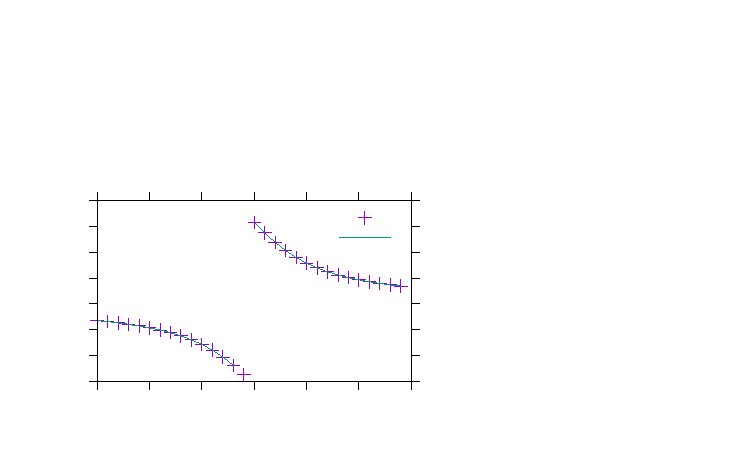
\includegraphics{plot-cairo4}}%
    \gplfronttext
  \end{picture}%
\endgroup

\caption{Comparison between the calculated modified arccotangent function using differential equation found in "myarccot2.c" and the arccot function from the math.h library, by calculation of arctan of the inverse value.}
\label{fig-acot2}
\end{figure}

\section{Implementation and Solution}
The implementation is done just as in the error-function exercise, by a solution of the differential equation, as represented by equation \eqref{eq:arctan} and \eqref{eq:arccot}. For $\arctan$ one can solve the differenial equation direcly, since the integration limits is from $0$ to $x$. This can be done just as in the error-function exercise. For the $\mathrm{arccot}$ function, if one wants to implement the same method direcly, by starting from $0$, you would need to reduce equation \eqref{eq:arccot}. This can be done avoiding the singularity at $z=\i$, and using equation \eqref{eq:arctan} by
\begin{align}
\mathrm{arccot}(x) &= \int_x^\infty \frac{1}{z^2 + 1} dz \nonumber\\
&= \int_0^\infty \frac{1}{z^2 + 1} dz - \int_0^x \frac{1}{z^2 + 1} dz \nonumber \\
&= \arctan(\infty) - \arctan(0) - \int_0^x \frac{1}{z^2 + 1} dz \nonumber \\
&=  \frac{\pi}{2} - 0 - \int_0^x \frac{1}{z^2 + 1} dz \nonumber \\
&=  \frac{\pi}{2} + \int_0^x - \frac{1}{z^2 + 1} dz \label{eq:arccot2} 
\end{align}
This is implemented by the well known $\mathrm{GSL\_ ode\_ iv2.h}$ library. The differential equations solved is given in equation \eqref{eq:arctan} and \eqref{eq:arccot2}, and are very similar except for a change of sign and an offset. The funciton is included as the $\mathrm{sys.function}$. The $\mathrm{sys.jacobian}$ is set to $\mathrm{NULL}$ as well as the $\mathrm{sys.params}$. The dimension of the problem is only one, and the driver applied is the generally accurate $\mathrm{gsl\_odeiv2\_step\_rkf45}$. For the $\mathrm{arctan}$ we know the initial conditions $\arctan(0) = 0$, and due to equation \eqref{eq:sumrelation} we therefore have start-condition for $\mathrm{arccot}(0)=\pi /2$. From here on, we just advance in steps defined by the driver, until we reach the desired value. Due to the fact that both of the $\arctan$ and $\mathrm{arccot}$ are odd functions, we can reduce the numerical calculation to positive values, by the identitiy of odd functions
\begin{align}
\arctan(-t) &= - \arctan(t), \\
\mathrm{arccot}(-t) &= - \mathrm{arccot}(t).
\end{align} 

Buy this method, the plots on figure \ref{fig-atan} and \ref{fig-acot} are made and compared to the tabular functions defined in the $\mathrm{math.h}$-library. Here we for the undefined $\mathrm{arccot}$ function define it using $\mathrm{math.h}$ as:
\begin{equation}
\mathrm{arccot}(x) = \arctan \left( \frac{1}{x} \right)
\end{equation}

On the second two figures \ref{fig-atan2} and \ref{eq:arccot2}, we have implemented a check for whether the argument in the functions are above or below $1$, to satisfy the condition to solve $\arctan(x)$, if $x \leq 1$, and $\mathrm{arccot}(x)$ for $x>1$, and compensate by formula \eqref{eq:sumrelation}. There is no visible difference between the ordinary solutions \ref{fig-atan} and \ref{eq:arccot} compared to the modified versions in figure \ref{fig-atan2} and \ref{eq:arccot2}. To show the differences between the two figures, I have tried to use a less accurate stepping function, and allowing the step-function to give higher errors, but the driver seems to compensate, and therefore a visible difference has not been shown here in the report. However the modified functions are denoted in the files by a $2$, and give the correct results. 


As an optional task, one should argue whether the ideal point to switch integration routine, should be just at the argument $x=1$. This is simple to show, since the numerical differential equation solver for the two equations only differ by a sign, making them equally difficult to solve for the driver. Thereby since the functions respond equally to the driver, the function, which returns the lowest output must be the most accurate, since the computing accuracy is best at small numbers. Thereby as $\arctan (0)= 0$ and $\mathrm{arccot}(0) = \pi /2$, we must for small $x$ have highest accuracy evolving $\arctan$. At high $x$, we will have $\arctan$ approacing $\pi /2$ and according to equation \eqref{eq:sumrelation} have $\mathrm{arccot}$ approaching $0$, making the $\mathrm{arccot}$ be the most accurate. Since they both converge with axcactly the same ratio, one would find the ideal point to swich integration routine, to be exactly when the two functions are equal, where they due to equation \eqref{eq:sumrelation} both return $\pi/4$. This happens excactly at

\begin{equation}
\arctan(1) = \mathrm{arccot}(1) = \frac{\pi}{4}
\end{equation}

Therefore at $x=1$ we have the ideal place to change integration routine. This conclusion as well as the implementation of both the initial code, and the modified code ends this project.  
\end{document}
